% !TEX program = xelatex
% !TEX encoding = UTF-8 Unicode
%% EE588 AWG 项目演讲稿（中文版 v3）
%% 15页幻灯片，10分钟演讲
%% 编译：xelatex（需运行两次）

\PassOptionsToPackage{table}{xcolor}
\documentclass[aspectratio=169,10pt]{beamer}

\usepackage{fontspec}
\setsansfont{STHeiti}[Script=CJK]
\setmainfont{STHeiti}[Script=CJK]
\XeTeXlinebreaklocale "zh"
\XeTeXlinebreakskip = 0pt plus 1pt

\usetheme{Madrid}
\usecolortheme{seahorse}
\setbeamertemplate{navigation symbols}{}
\setbeamertemplate{footline}[frame number]

\usepackage{graphicx}
\usepackage{booktabs}
\usepackage{amsmath}
\usepackage{tikz}
\usepackage{array}
\usepackage{multirow}

\usetikzlibrary{decorations.pathmorphing,arrows.meta,patterns,positioning}

\definecolor{uw_purple}{RGB}{51,0,111}
\definecolor{uw_gold}{RGB}{232,211,162}
\definecolor{good_green}{RGB}{0,153,76}
\definecolor{passing_blue}{RGB}{0,102,204}
\definecolor{poor_red}{RGB}{204,0,0}
\definecolor{si_blue}{RGB}{70,130,180}
\definecolor{sio2_gray}{RGB}{210,215,220}

\setbeamercolor{frametitle}{bg=uw_purple,fg=white}
\setbeamercolor{title}{bg=uw_purple,fg=white}
\setbeamercolor{structure}{fg=uw_purple}

\title[EE588 AWG]{C波段 4通道阵列波导光栅（AWG）\\波长解复用器设计与仿真}
\subtitle{EE588 期末项目}
\author{Donald Luo \and Yangyuan Yin}
\institute{华盛顿大学（University of Washington）}
\date{\today}

\begin{document}

% ── 第1页：标题 ──────────────────────────────────────────────────────────────
\begin{frame}
  \titlepage
\end{frame}

% ── 第2页：动机一——数据中心带宽挑战 ───────────────────────────────────────────
\begin{frame}{动机一：数据中心带宽挑战}
  \begin{columns}[T]
    \column{0.56\textwidth}
      \textbf{全球数据中心流量正在爆炸式增长}
      \begin{itemize}\setlength\itemsep{3pt}
        \item 2021年达 \textbf{20.6 ZB/年}，年增长率约 25\%\footnotemark[1]
        \item 77\% 的流量留在数据中心内部（服务器间通信）
        \item 继续堆铜线已触碰物理极限：\\
              {\small 电阻发热、电磁串扰、能耗过高}
      \end{itemize}
      \vspace{0.5em}
      \textbf{光互联是唯一可扩展的出路}
      \begin{itemize}\setlength\itemsep{3pt}
        \item 400GbE / 800GbE 标准已强制要求 WDM 光模块\footnotemark[2]
        \item \textbf{WDM（波分复用）}：把 $N$ 路信号"染"成不同颜色，混合在一根光纤里传
        \item 接收端需要\textbf{波长解复用器}把各颜色分开，送到各自接收器
      \end{itemize}
    \column{0.41\textwidth}
      \begin{block}{解复用器做什么}
        \centering
        \begin{tikzpicture}[scale=0.82]
          \draw[very thick,blue!60,->] (-1.8,0)--(-0.05,0);
          \node[above,font=\tiny] at (-0.9,0.05) {混合波长 $\lambda_1\!\cdots\!\lambda_4$};
          \fill[uw_purple!20,rounded corners=3pt] (0,-1.1) rectangle (1.3,1.1);
          \node[font=\scriptsize,align=center] at (0.65,0) {解复用器\\（AWG）};
          \draw[red,thick,->] (1.3,0.75)--(2.4,0.75);
          \node[right,red,font=\tiny] at (2.4,0.75) {$\lambda_1$};
          \draw[orange,thick,->] (1.3,0.25)--(2.4,0.25);
          \node[right,orange,font=\tiny] at (2.4,0.25) {$\lambda_2$};
          \draw[green!60!black,thick,->] (1.3,-0.25)--(2.4,-0.25);
          \node[right,green!60!black,font=\tiny] at (2.4,-0.25) {$\lambda_3$};
          \draw[blue,thick,->] (1.3,-0.75)--(2.4,-0.75);
          \node[right,blue,font=\tiny] at (2.4,-0.75) {$\lambda_4$};
        \end{tikzpicture}\\[4pt]
        一路混合光进，四路分色光出。\\
        \textbf{这就是我们要做的器件。}
      \end{block}
  \end{columns}
  \footnotetext[1]{\tiny Cisco Annual Internet Report 2022.}
  \footnotetext[2]{\tiny D.~A.~B.~Miller, \textit{Proc.\ IEEE} 88, 728--749 (2000).}
\end{frame}

% ── 第3页：动机二——为什么选硅基AWG ────────────────────────────────────────────
\begin{frame}{动机二：为什么选硅基阵列波导光栅（AWG）？}
  \begin{columns}[T]
    \column{0.50\textwidth}
      \textbf{AWG：芯片级解复用器的工业标准}\footnotemark[3]
      \begin{itemize}\setlength\itemsep{3pt}
        \item 1988 年由 Smit 首次提出；现已内置于每台相干光收发器
        \item 通道数 4--96，插入损耗 $<$2\,dB（商用水平）
        \item 本质：\emph{相控阵空间滤波器}——无需移动部件
      \end{itemize}
      \vspace{0.4em}
      \textbf{为什么用硅（SOI 平台）？}\footnotemark[4]
      \begin{itemize}\setlength\itemsep{3pt}
        \item CMOS 兼容——可在现有半导体工厂直接流片
        \item Si/SiO$_2$ 折射率差巨大（$\Delta n \approx 2.0$）\\
              $\Rightarrow$ 弯曲半径 $<$10\,$\mu$m，器件面积 $\sim$mm$^2$
        \item 可与锗光探测器、硅调制器集成在同一芯片
      \end{itemize}
    \column{0.47\textwidth}
      \begin{block}{本项目 4 通道 C 波段目标（ITU-T G.694.1\footnotemark[5]）}
        \centering\small
        \renewcommand{\arraystretch}{1.15}
        \begin{tabular}{cc}
          \toprule
          通道 & 中心波长（nm） \\
          \midrule
          通道 1 & 1547.6 \\
          通道 2 & 1549.2 \\
          通道 3 & 1550.8 \\
          通道 4 & 1552.4 \\
          \midrule
          \multicolumn{2}{c}{间距 1.6\,nm $\approx$ 200\,GHz（DWDM）}\\
          \bottomrule
        \end{tabular}
      \end{block}
      \vspace{0.3em}
      \small 平台：500\,nm\,$\times$\,220\,nm 硅条形波导 / SiO$_2$。
  \end{columns}
  \footnotetext[3]{\tiny M.~K.~Smit \& C.~van Dam, \textit{IEEE JSTQE} 2, 236 (1996).}
  \footnotetext[4]{\tiny L.~Chrostowski \& M.~Hochberg, \textit{Silicon Photonics Design}, Cambridge, 2015.}
  \footnotetext[5]{\tiny ITU-T G.694.1, DWDM frequency grid, 2012.}
\end{frame}

% ── 第4页：AWG 物理结构 ───────────────────────────────────────────────────────
\begin{frame}{AWG 物理结构：从波导到芯片}
  \begin{columns}[T]
    \column{0.44\textwidth}
      \textbf{第一步：波导横截面}\\[4pt]
      \begin{center}
      \begin{tikzpicture}[scale=1.05, font=\tiny]
        \fill[sio2_gray!70] (-1.7,-0.75) rectangle (1.7,-0.18);
        \node at (0,-0.48) {SiO$_2$ 衬底，$n{=}1.44$};
        \fill[si_blue!70] (-0.28,-0.18) rectangle (0.28,0.18);
        \node[white,font=\bfseries\tiny] at (0,0) {Si 核心};
        \fill[sio2_gray!30] (-1.7,0.18) rectangle (1.7,0.62);
        \node at (0,0.40) {SiO$_2$ 包层，$n{=}1.44$};
        \draw[red!80,very thick,domain=-0.72:0.72,samples=60]
          plot(\x,{0.36*exp(-18*\x*\x)});
        \node[red!70] at (1.05,0.38) {TE 模式};
        \draw[black!50,<->,thin] (-0.28,-0.56)--(0.28,-0.56)
          node[midway,below,black!70] {500\,nm};
        \draw[black!50,<->,thin] (0.42,-0.18)--(0.42,0.18)
          node[midway,right,black!70] {220\,nm};
        \draw[black!30,dashed,thin] (-0.28,-0.18)--(-0.28,-0.50)
          (0.28,-0.18)--(0.28,-0.50);
        \node[above,font=\tiny\itshape] at (0,0.65) {光被全内反射限制在 Si 核心中传播};
      \end{tikzpicture}
      \end{center}
      \vspace{0.3em}
      \small $n_{\mathrm{Si}}=3.48 \gg n_{\mathrm{SiO_2}}=1.44$\;$\Rightarrow$\;光不外泄。

    \column{0.53\textwidth}
      \textbf{第二步：AWG 芯片俯视图}\\[4pt]
      \begin{center}
      \begin{tikzpicture}[scale=0.85, font=\tiny]
        \draw[blue!70,very thick,->] (-4.2,0)--(-3.3,0);
        \node[above,blue!70,align=center] at (-3.75,0.05) {输入\\（混合波长）};
        \fill[cyan!25] (-3.3,-0.8)--(-2.2,-1.4)--(-2.2,1.4)--(-3.3,0.8)--cycle;
        \node[align=center] at (-2.75,0) {FPR 1\\（星形\\耦合器）};
        \foreach \k/\ys/\ye/\ext in {
          1/1.1/0.9/0.0,
          2/0.65/0.55/0.15,
          3/0.22/0.18/0.30,
          4/-0.22/-0.18/0.45,
          5/-0.65/-0.55/0.60,
          6/-1.1/-0.9/0.75}{
          \draw[uw_purple!60,thick]
            (-2.2,\ys) -- (-1.5,\ys)
            -- (-1.5,{\ys-\ext*0.4}) -- (-0.8,{\ys-\ext*0.4}) -- (-0.8,\ys)
            -- (-0.1,\ye);
        }
        \node[below,align=center] at (-1.15,-1.35) {16根阵列臂\\各增加 $\Delta L$ 长度};
        \fill[cyan!25] (-0.1,-1.4)--(1.0,-0.8)--(1.0,0.8)--(-0.1,1.4)--cycle;
        \node[align=center] at (0.45,0) {FPR 2\\（输出\\路由器）};
        \draw[red,very thick,->] (1.0,0.6)--(2.0,0.6);
        \node[right,red] at (2.0,0.6) {$\lambda_1$};
        \draw[orange,very thick,->] (1.0,0.2)--(2.0,0.2);
        \node[right,orange] at (2.0,0.2) {$\lambda_2$};
        \draw[green!70!black,very thick,->] (1.0,-0.2)--(2.0,-0.2);
        \node[right,green!70!black] at (2.0,-0.2) {$\lambda_3$};
        \draw[blue,very thick,->] (1.0,-0.6)--(2.0,-0.6);
        \node[right,blue] at (2.0,-0.6) {$\lambda_4$};
        \draw[black!50] (-4.0,-1.6)--(-2.0,-1.6)
          node[midway,below,black!60] {$\sim$0.5\,mm};
      \end{tikzpicture}
      \end{center}
  \end{columns}
\end{frame}

% ── 第5页：AWG 如何分色 ───────────────────────────────────────────────────────
\begin{frame}{AWG 如何分色：相位控制干涉}
  \begin{columns}[T]
    \column{0.46\textwidth}
      \textbf{核心思想：不同臂长 = 不同相位延迟}
      \begin{center}
      \begin{tikzpicture}[scale=0.9, font=\tiny]
        \node[left] at (-0.1,1.5) {臂 0};
        \node[left] at (-0.1,0.5) {臂 1};
        \node[left] at (-0.1,-0.5) {臂 2};
        \node[left] at (-0.1,-1.5) {臂 3};
        \draw[uw_purple!70,thick] (0,1.5) -- (3.5,1.5);
        \draw[uw_purple!70,thick] (0,0.5) -- (0.8,0.5)
          -- (0.8,0.1) -- (1.8,0.1) -- (1.8,0.5) -- (3.5,0.5);
        \draw[uw_purple!70,thick] (0,-0.5) -- (0.8,-0.5)
          -- (0.8,-1.1) -- (2.2,-1.1) -- (2.2,-0.5) -- (3.5,-0.5);
        \draw[uw_purple!70,thick] (0,-1.5) -- (0.8,-1.5)
          -- (0.8,-2.1) -- (2.6,-2.1) -- (2.6,-1.5) -- (3.5,-1.5);
        \node[right] at (3.5,1.5) {$\phi_0$};
        \node[right] at (3.5,0.5) {$\phi_0{+}\beta\Delta L$};
        \node[right] at (3.5,-0.5) {$\phi_0{+}2\beta\Delta L$};
        \node[right] at (3.5,-1.5) {$\phi_0{+}3\beta\Delta L$};
        \draw[<->,red,thin] (1.82,0.1)--(1.82,-1.1)
          node[midway,right,red] {$\Delta L$};
        \node[above,font=\scriptsize,blue!70] at (1.5,1.7)
          {\textit{每根臂比上一根多走 $\Delta L$}};
      \end{tikzpicture}
      \end{center}

    \column{0.51\textwidth}
      \textbf{结果：相位倾斜方向随波长变化}
      \begin{center}
      \begin{tikzpicture}[scale=0.85, font=\tiny]
        \fill[cyan!20] (0,-2.0) rectangle (0.6,2.0);
        \node[rotate=90,font=\scriptsize] at (0.3,0) {FPR 2};
        \draw[red!70,thick] (0.7,1.6)--({0.7+0.3},0.6);
        \draw[red!70,thick] (1.1,1.6)--({1.1+0.3},0.6);
        \draw[red!70,thick] (1.5,1.6)--({1.5+0.3},0.6);
        \node[red!70] at (2.0,1.2) {$\lambda_1$};
        \draw[red!70,very thick,->] (1.5,1.1)--(2.5,1.5);
        \draw[orange!80,thick] (0.7,0.7)--({0.7+0.15},-0.1);
        \draw[orange!80,thick] (1.1,0.7)--({1.1+0.15},-0.1);
        \draw[orange!80,thick] (1.5,0.7)--({1.5+0.15},-0.1);
        \node[orange!80] at (2.0,0.3) {$\lambda_2$};
        \draw[orange!80,very thick,->] (1.5,0.3)--(2.5,0.3);
        \draw[green!60!black,thick] (0.7,-0.3)--({0.7-0.1},-1.1);
        \draw[green!60!black,thick] (1.1,-0.3)--({1.1-0.1},-1.1);
        \draw[green!60!black,thick] (1.5,-0.3)--({1.5-0.1},-1.1);
        \node[green!60!black] at (2.0,-0.7) {$\lambda_3$};
        \draw[green!60!black,very thick,->] (1.5,-0.6)--(2.5,-0.9);
        \fill[gray!30] (2.5,-2.0) rectangle (2.7,2.0);
        \draw[red,very thick] (2.5,1.5)--(3.4,1.5);
        \draw[orange,very thick] (2.5,0.3)--(3.4,0.3);
        \draw[green!60!black,very thick] (2.5,-0.9)--(3.4,-0.9);
        \node[above,font=\scriptsize] at (1.5,2.0)
          {\textit{相同相位倾斜方向 $\Rightarrow$ 不同汇聚位置}};
      \end{tikzpicture}
      \end{center}
      \vspace{-2pt}
      \small\textbf{公式：} $\Delta L = m\lambda_0/n_g$\quad
      $\Rightarrow$\quad 在 $\lambda_0$ 处：所有臂恰好积累 $m$ 个完整相位周期。\\
      $\lambda\!\neq\!\lambda_0$ 时：相位差的小数部分使焦点向一侧偏移。
  \end{columns}
\end{frame}

% ── 第6页：项目 vs 商用产品 ──────────────────────────────────────────────────
\begin{frame}{我们的学术仿真 vs 商用硅基 AWG 产品}
  \begin{columns}[T]
    \column{0.50\textwidth}
      \small
      \renewcommand{\arraystretch}{1.30}
      \begin{tabular}{lcc}
        \toprule
        \textbf{指标} & \textbf{商用产品} & \textbf{本项目} \\
        \midrule
        工艺平台 & SOI 220\,nm & SOI 220\,nm \checkmark \\
        通道数 & 4--96 & 4 \\
        插入损耗 & $<$2\,dB & 3\,dB（模型） \\
        串扰 & $<$-30\,dB & -13.7\,dB（模型） \\
        流片成本 & \$\$\$/芯片 & 仅需仿真 \checkmark \\
        设计开放？ & 专有 & \textbf{完全公开} \checkmark \\
        系统优化？ & 固定产品 & \textbf{+15\% (N=24)} \checkmark \\
        \bottomrule
      \end{tabular}

      \vspace{0.5em}
      \begin{alertblock}{\small 为什么插损/串扰有差距？}
        \small 我们的 2D 简化模型省去了弯曲损耗、
        三维模式失配和制造粗糙度——
        完整 3D FDTD 可以大幅缩小这个差距。
      \end{alertblock}

    \column{0.47\textwidth}
      \begin{block}{本项目的\emph{独特贡献}}
        \begin{enumerate}\small\setlength\itemsep{4pt}
          \item \textbf{端到端的完整记录流程}\\
                MODE $\to$ 参数推导 $\to$ FDTD $\to$ 优化，\\
                所有步骤从第一原理可重现
          \item \textbf{系统性臂数研究}\\
                首次证明 N: 16$\to$24 使平均主输出占比\\
                提升 \textbf{+15\%}，优于纯几何调参
          \item \textbf{低成本验证框架}\\
                不到完整三维成本的 1\%，\\
                即可证明波长路由效果
          \item \textbf{学术方法论基准}\\
                为后续 Rowland 圆或逆向设计\\
                AWG 研究提供基准
        \end{enumerate}
      \end{block}
  \end{columns}
\end{frame}

% ── 第7页：三层仿真策略 ──────────────────────────────────────────────────────
\begin{frame}{三层仿真策略}
  \begin{center}
  \begin{tikzpicture}[scale=0.88, font=\small,
      box/.style={draw=uw_purple!60, fill=uw_purple!8, rounded corners=4pt,
                  minimum width=3.4cm, minimum height=0.9cm, align=center}]
    \node[box] (L1) at (0, 2.2)
      {\textbf{层次 1：MODE 求解器}\\{\tiny Tidy3D 云端}};
    \node[right=0.3cm of L1, font=\footnotesize, text width=6.8cm]
      {提取 $n_\text{eff}$、$n_g$。回答：\textit{波导的光学常数是什么？}};
    \node[box, fill=uw_gold!20, draw=uw_gold!70!black] (L2) at (0, 0.7)
      {\textbf{层次 2：阵列因子模型}\\{\tiny 本地运行，免费}};
    \node[right=0.3cm of L2, font=\footnotesize, text width=6.8cm]
      {解析频谱公式。回答：\textit{通道方案是否合理？}};
    \node[box, fill=good_green!10, draw=good_green!60] (L3) at (0,-0.8)
      {\textbf{层次 3：2D 有效折射率 FDTD}\\{\tiny Tidy3D 云端}};
    \node[right=0.3cm of L3, font=\footnotesize, text width=6.8cm]
      {FPR 区真实麦克斯韦求解。回答：\textit{光是否真的路由到了正确端口？}};
    \draw[->,thick,uw_purple!50] (L1.south)--(L2.north);
    \draw[->,thick,uw_purple!50] (L2.south)--(L3.north);
    \node[box, fill=gray!10, draw=gray!40, font=\small\itshape] (L4) at (0,-2.3)
      {层次 4：完整 3D FDTD——未做（超出课程范围）};
    \draw[->,dashed,gray!50] (L3.south)--(L4.north);
  \end{tikzpicture}
  \end{center}
  \vspace{-4pt}
  \small\textit{每个层次解答一个具体的设计问题，保真度逐步提升。
  层次 3 已能证明波长路由效果，因此在此停止。}
\end{frame}

% ── 第8页：波导 MODE 分析 ─────────────────────────────────────────────────────
\begin{frame}{第一阶段 — 波导 MODE 模式分析}
  \begin{columns}[T]
    \column{0.43\textwidth}
      \textbf{硅/二氧化硅条形波导，高度 $h=220$\,nm（固定 SOI 工艺）}\\[5pt]
      \small
      \begin{tabular}{ccc}
        \toprule
        宽度 & $n_\text{eff}$ & $n_g$ \\
        \midrule
        400\,nm & 2.228 & 4.245 \\
        450\,nm & 2.353 & 4.144 \\
        \rowcolor{uw_gold!60}
        \textbf{500\,nm\,$^\star$} & \textbf{2.445} & \textbf{4.051} \\
        550\,nm & 2.513 & 3.975 \\
        600\,nm & 2.566 & 3.914 \\
        \bottomrule
      \end{tabular}
      \vspace{6pt}

      \small$^\star$ \textit{选定基准}：折射率居中，准单模，SOI 标准尺寸。\\[4pt]
      \textbf{规律：} 宽度增大 $\Rightarrow$ $n_\text{eff}\uparrow$，$n_g\downarrow$。\\[4pt]
      $n_g = 4.051$ 直接代入 AWG 设计：\\
      \centerline{$\Delta L = m\lambda_0/n_g = 30.99\,\mu$m}

    \column{0.54\textwidth}
      \begin{center}
        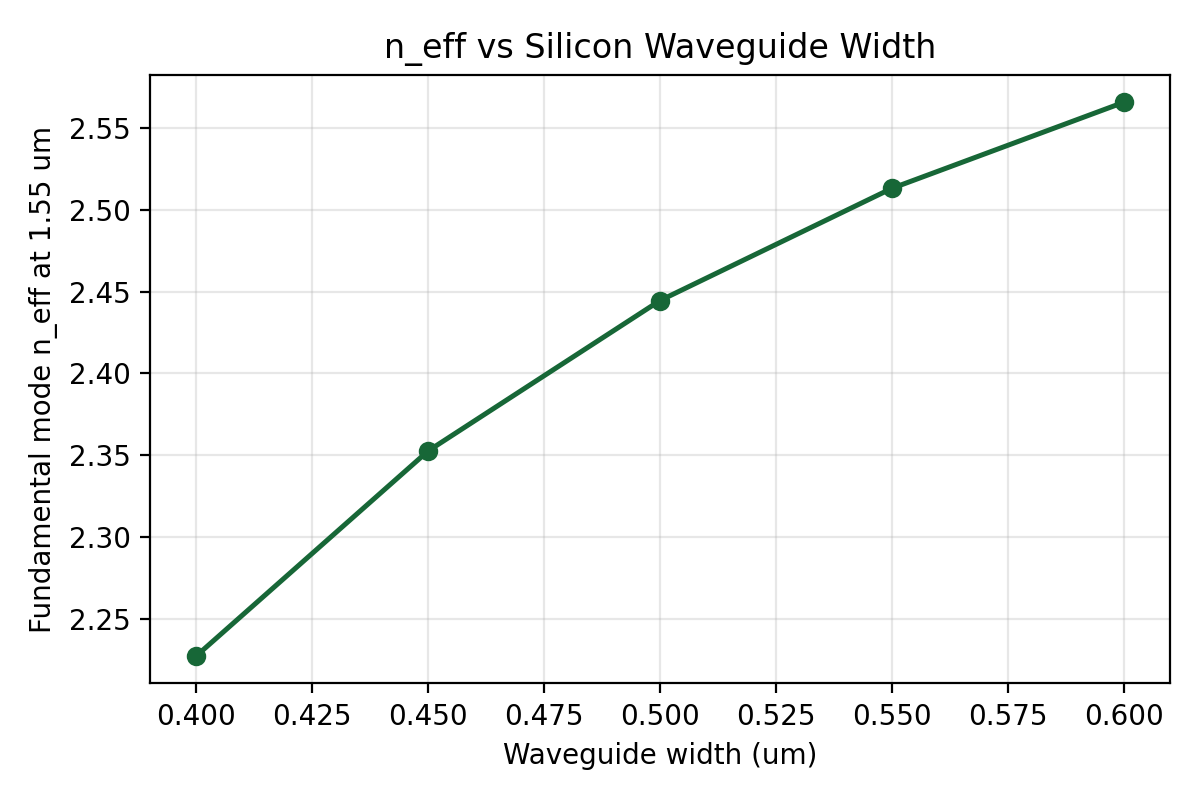
\includegraphics[width=\linewidth]{results/figures/neff_vs_width.png}
        {\footnotesize $n_\text{eff}$ 与 $n_g$ 随波导宽度变化（1550\,nm）}
      \end{center}
  \end{columns}
\end{frame}

% ── 第9页：AWG 初始参数设计 ──────────────────────────────────────────────────
\begin{frame}{第二阶段 — AWG 初始参数设计}
  \begin{columns}[T]
    \column{0.43\textwidth}
      \small\textbf{参数推导链（从 MODE 结果出发）：}\\[4pt]
      \renewcommand{\arraystretch}{1.18}
      \begin{tabular}{ll}
        \toprule
        参数 & 数值 \\
        \midrule
        中心波长 $\lambda_0$ & 1550\,nm \\
        通道间距 & 1.6\,nm \\
        目标 FSR & 19.2\,nm \\
        衍射级次 $m$ & 81 \\
        实际 FSR & 19.14\,nm \\
        $\Delta L = m\lambda_0/n_g$ & 30.99\,$\mu$m \\
        \midrule
        输入/输出/臂数 & 1/4/16 \\
        FPR 长度 & 55\,$\mu$m \\
        阵列间距（初始） & 1.50\,$\mu$m \\
        输出间距（初始） & 2.00\,$\mu$m \\
        \bottomrule
      \end{tabular}

    \column{0.54\textwidth}
      \begin{center}
        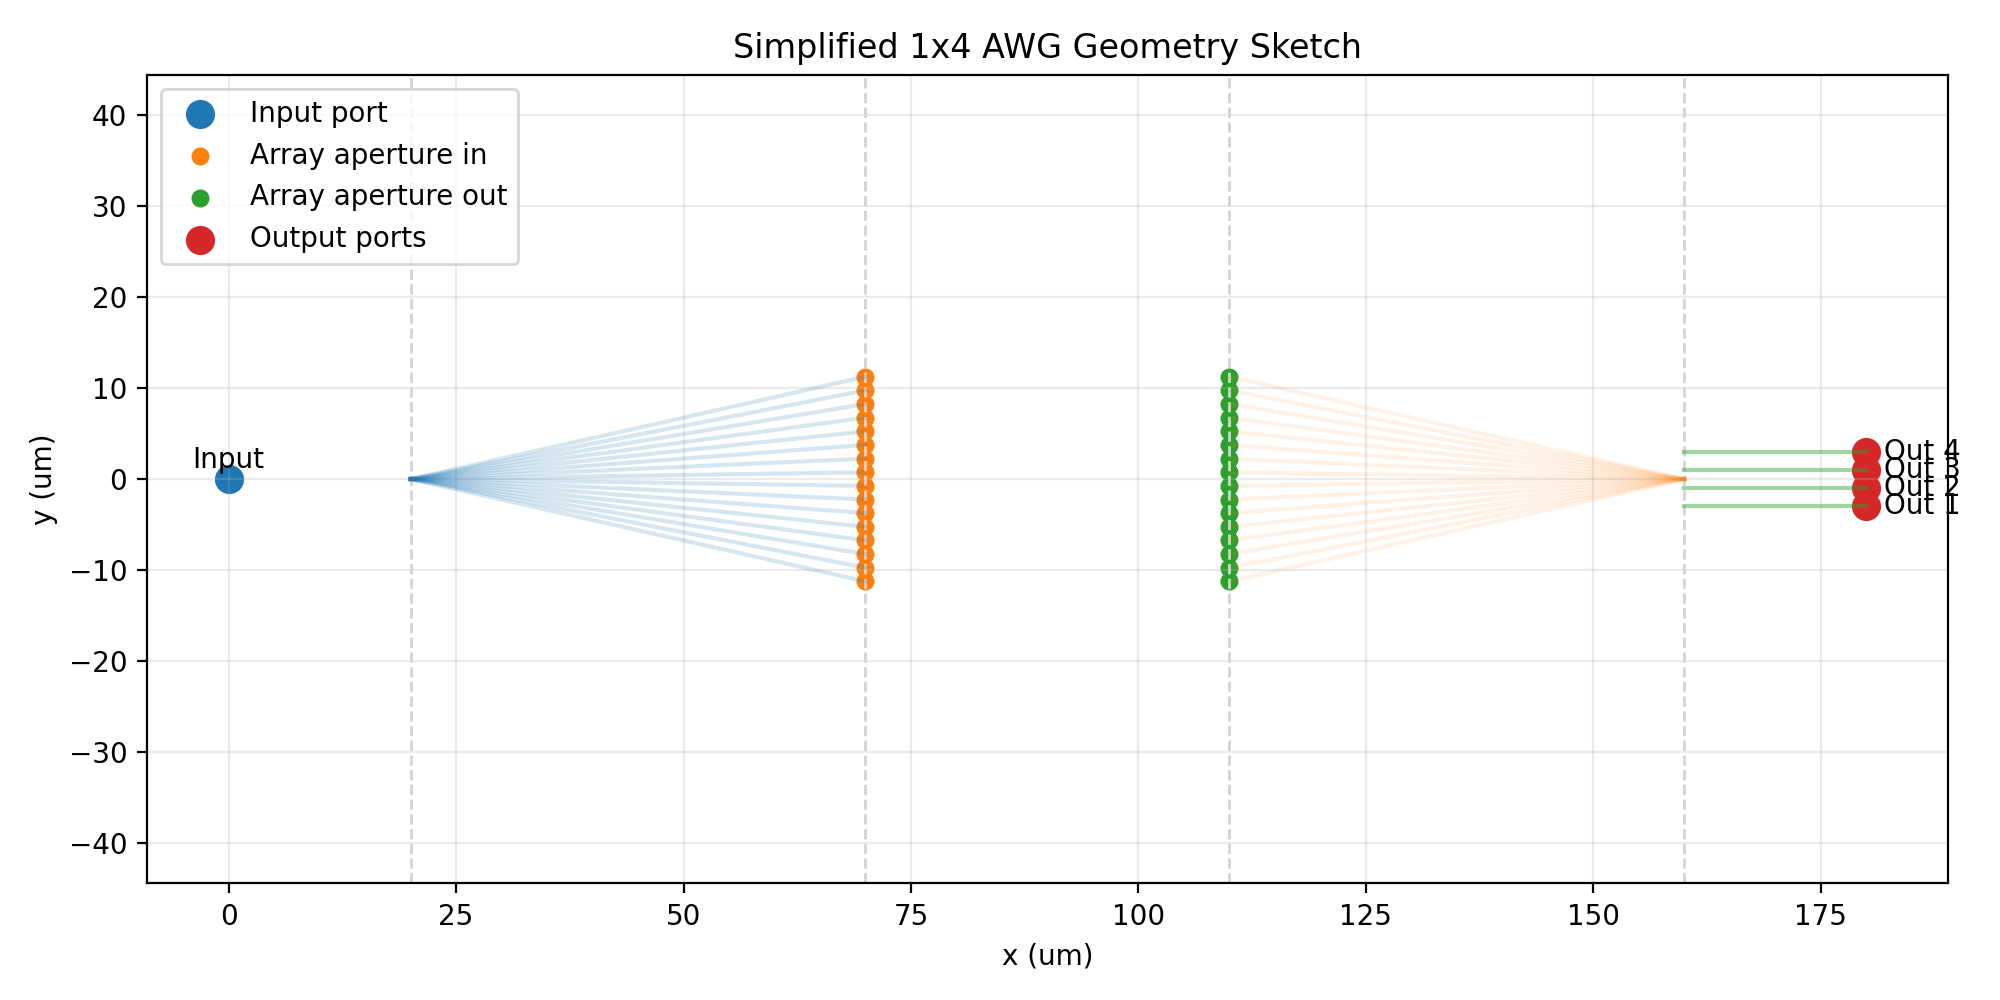
\includegraphics[width=\linewidth]{results/figures/simplified_awg_geometry_layout.png}
        {\footnotesize 简化版 AWG 几何布局（1输入，4输出，16根臂）}
      \end{center}
  \end{columns}
\end{frame}

% ── 第10页：简化频谱模型 ─────────────────────────────────────────────────────
\begin{frame}{第三阶段（A）— 阵列因子频谱模型（零计算成本）}
  \begin{columns}[T]
    \column{0.43\textwidth}
      \textbf{解析公式：}
      \[
        T(\lambda) = T_\text{峰}\!
        \underbrace{\left(\frac{\sin(N\phi/2)}{N\sin(\phi/2)}\right)^{\!2}}_{\text{阵列因子（干涉图样）}}
        \!\cdot\!
        \underbrace{e^{-\delta\lambda^2/2\sigma^2}}_{\text{高斯包络（耦合效率）}}
      \]
      $\phi\!=\!2\pi\delta\lambda/\text{FSR}$，$N\!=\!16$，$\sigma\!=\!6$\,nm

      \vspace{0.5em}
      \begin{block}{\small 模型预测指标}
        \small
        \begin{tabular}{ll}
          插入损耗 & 3.0\,dB \\
          串扰 & $-13.7$\,dB \\
          3\,dB 带宽 & 1.06\,nm \\
          通道间距 & 1.60\,nm\;\checkmark \\
        \end{tabular}
      \end{block}
      \begin{alertblock}{\small 模型局限}
        \small 对称模型：4 个通道结果完全相同。\\
        实际器件：边缘通道插损更大。
      \end{alertblock}

    \column{0.54\textwidth}
      \begin{center}
        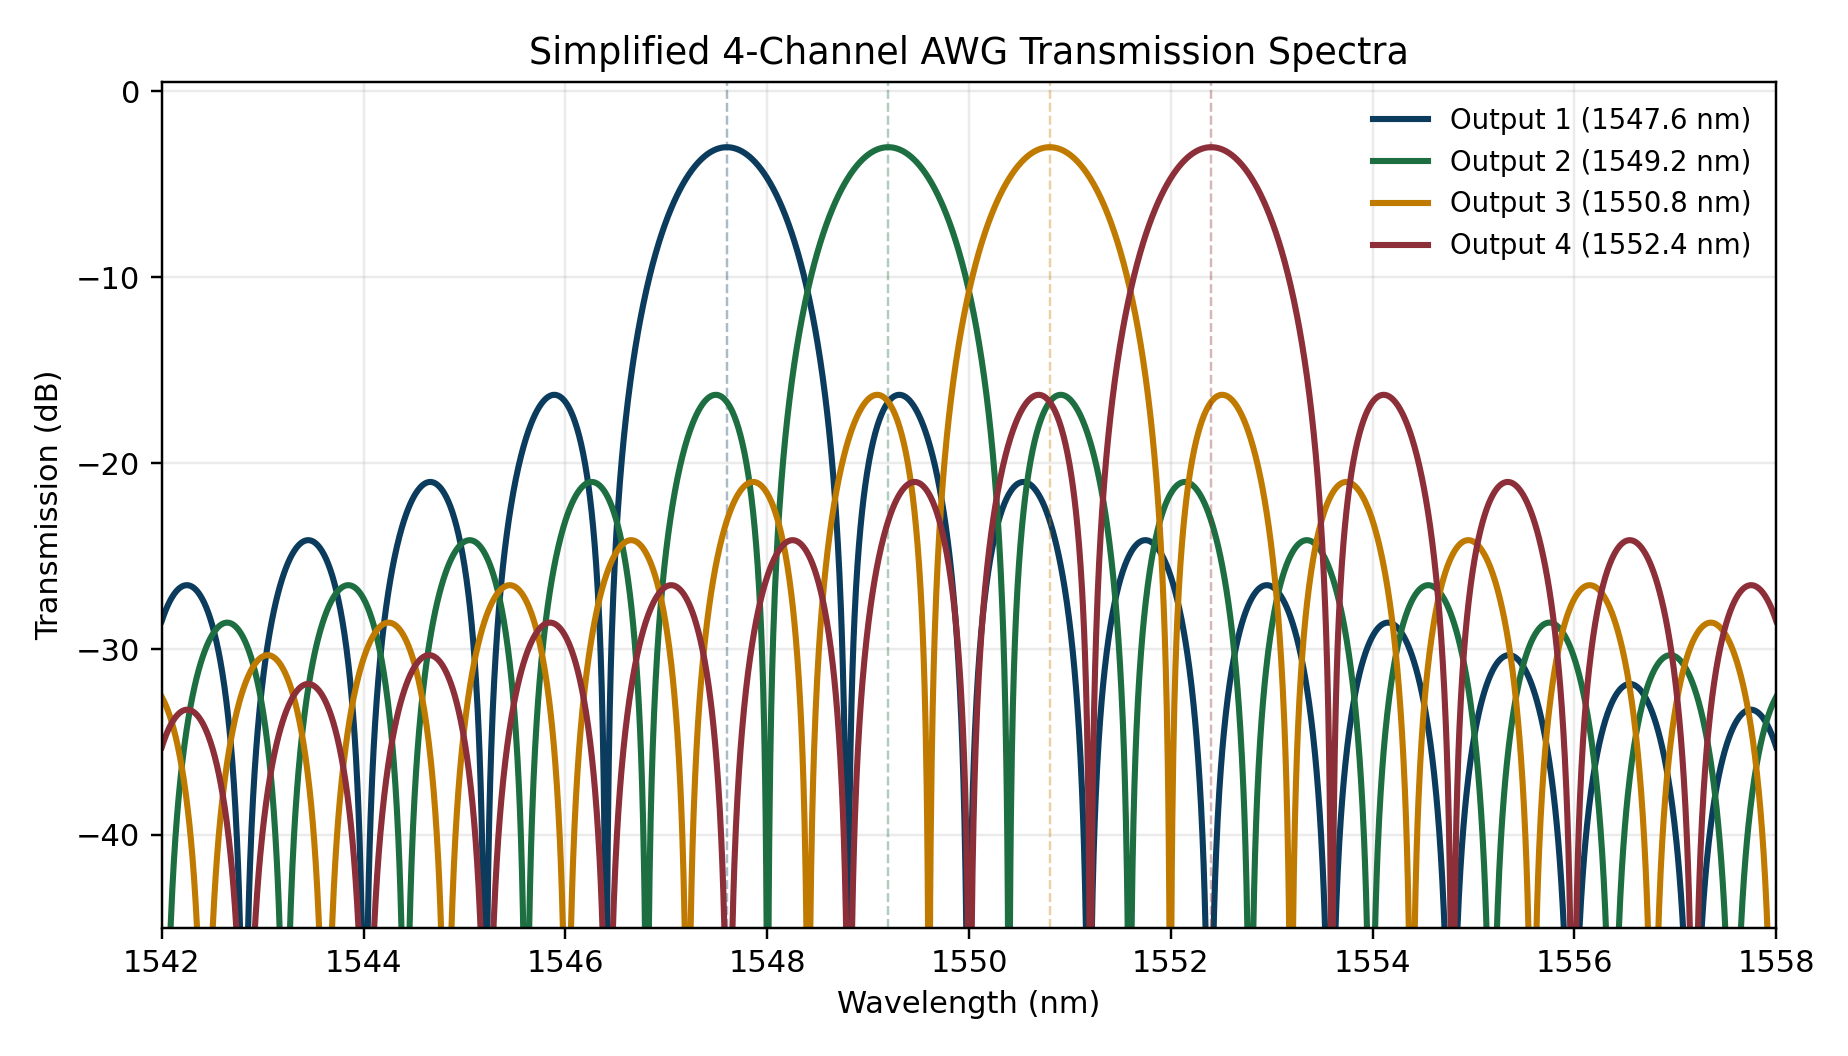
\includegraphics[width=\linewidth]{results/figures/awg_transmission_spectra.png}
        {\footnotesize 预测的 4 通道传输谱（1547.6 -- 1552.4\,nm）}
      \end{center}
  \end{columns}
\end{frame}

% ── 第11页：FDTD 验证设置与评级 ──────────────────────────────────────────────
\begin{frame}{第三阶段（B）— 2D FDTD 高保真器件级验证}
  \begin{columns}[T]
    \column{0.50\textwidth}
      \textbf{为什么用 2D 而不是完整 3D？}
      \begin{itemize}\small\setlength\itemsep{3pt}
        \item 完整 3D 器件（$\sim$2\,mm 长）成本过高
        \item \textbf{2D 有效折射率技巧：} 用 $n_\text{eff}$ 等效三维截面，压缩为二维
        \item 只对输出 FPR 区段做 FDTD；臂相位解析预设
        \item 节省 $\sim$100 倍计算量
      \end{itemize}
      \vspace{0.4em}
      \begin{tikzpicture}[scale=0.75, font=\tiny]
        \fill[cyan!15] (0,-0.8) rectangle (3.0,0.8);
        \node at (1.5,0) {FPR 平板（2D FDTD）};
        \draw[uw_purple!60,thick,->] (-1.2,0.55)--(-0.05,0.55);
        \node[left,uw_purple!60] at (-1.2,0.55) {臂 1: $\phi_1$};
        \draw[uw_purple!60,thick,->] (-1.2,0.18)--(-0.05,0.18);
        \node[left,uw_purple!60] at (-1.2,0.18) {臂 2: $\phi_2$};
        \draw[uw_purple!60,thick,->] (-1.2,-0.18)--(-0.05,-0.18);
        \node[left,uw_purple!60] at (-1.2,-0.18) {臂 3: $\phi_3$};
        \draw[uw_purple!60,thick,->] (-1.2,-0.55)--(-0.05,-0.55);
        \node[left,uw_purple!60] at (-1.2,-0.55) {臂 4: $\phi_4$};
        \draw[red,thick,->] (3.0,0.55)--(4.0,0.55);
        \draw[orange,thick,->] (3.0,0.18)--(4.0,0.18);
        \draw[green!60!black,thick,->] (3.0,-0.18)--(4.0,-0.18);
        \draw[blue,thick,->] (3.0,-0.55)--(4.0,-0.55);
        \node[below,align=center] at (1.5,-0.85)
          {16 路相位源 $\to$ 真实 FDTD $\to$ 4 路功率监测};
      \end{tikzpicture}

    \column{0.47\textwidth}
      \textbf{路由质量评级标准：}\\[4pt]
      \small
      \renewcommand{\arraystretch}{1.25}
      \begin{tabular}{lcc}
        \toprule
        等级 & 主输出占比 & 次/主比 \\
        \midrule
        \textcolor{good_green}{\textbf{优（Good）}} & $\geq 0.60$ & $\leq 0.50$ \\
        \textcolor{passing_blue}{\textbf{良（General）}} & $\geq 0.40$ & $\leq 0.80$ \\
        \textbf{合格（Passing）} & $\geq 0.30$ & $\leq 0.95$ \\
        \textcolor{poor_red}{\textbf{差（Poor）}} & \multicolumn{2}{c}{低于合格线} \\
        \bottomrule
      \end{tabular}
      \vspace{5pt}\\
      \footnotesize
      \textit{主输出占比}：最强端口功率/总功率（越高越好）\\[2pt]
      \textit{次/主比}：次强/最强（越低分离越干净）
  \end{columns}
\end{frame}

% ── 第12页：Baseline FDTD 结果 ────────────────────────────────────────────────
\begin{frame}{Baseline FDTD 验证——波长路由物理确认}
  \begin{columns}[T]
    \column{0.43\textwidth}
      \small\textbf{初始配置：} $N\!=\!16$，阵距 $1.5\,\mu$m，输出距 $2.0\,\mu$m\\[5pt]
      \renewcommand{\arraystretch}{1.25}
      \begin{tabular}{cccc}
        \toprule
        $\lambda$ & 主输出 & 占比 & 等级 \\
        \midrule
        1547.6\,nm & out\_3 & 0.390 & 合格 \\
        1549.2\,nm & out\_3 & 0.340 & 合格 \\
        1550.8\,nm & out\_4 & 0.328 & 合格 \\
        1552.4\,nm & out\_4 & 0.350 & 合格 \\
        \midrule
        \textbf{均值} & — & \textbf{0.352} & 合格 \\
        \bottomrule
      \end{tabular}
      \vspace{5pt}

      \begin{block}{\small 核心发现}
        \small 主输出端口随波长增加从 out\_3 $\to$ out\_4。\\[3pt]
        \textbf{波长依赖性路由在真实 FDTD 中确认}——\\
        这是麦克斯韦方程组的真实求解结果，\\
        不是数学模型的预测。
      \end{block}

    \column{0.54\textwidth}
      \begin{center}
        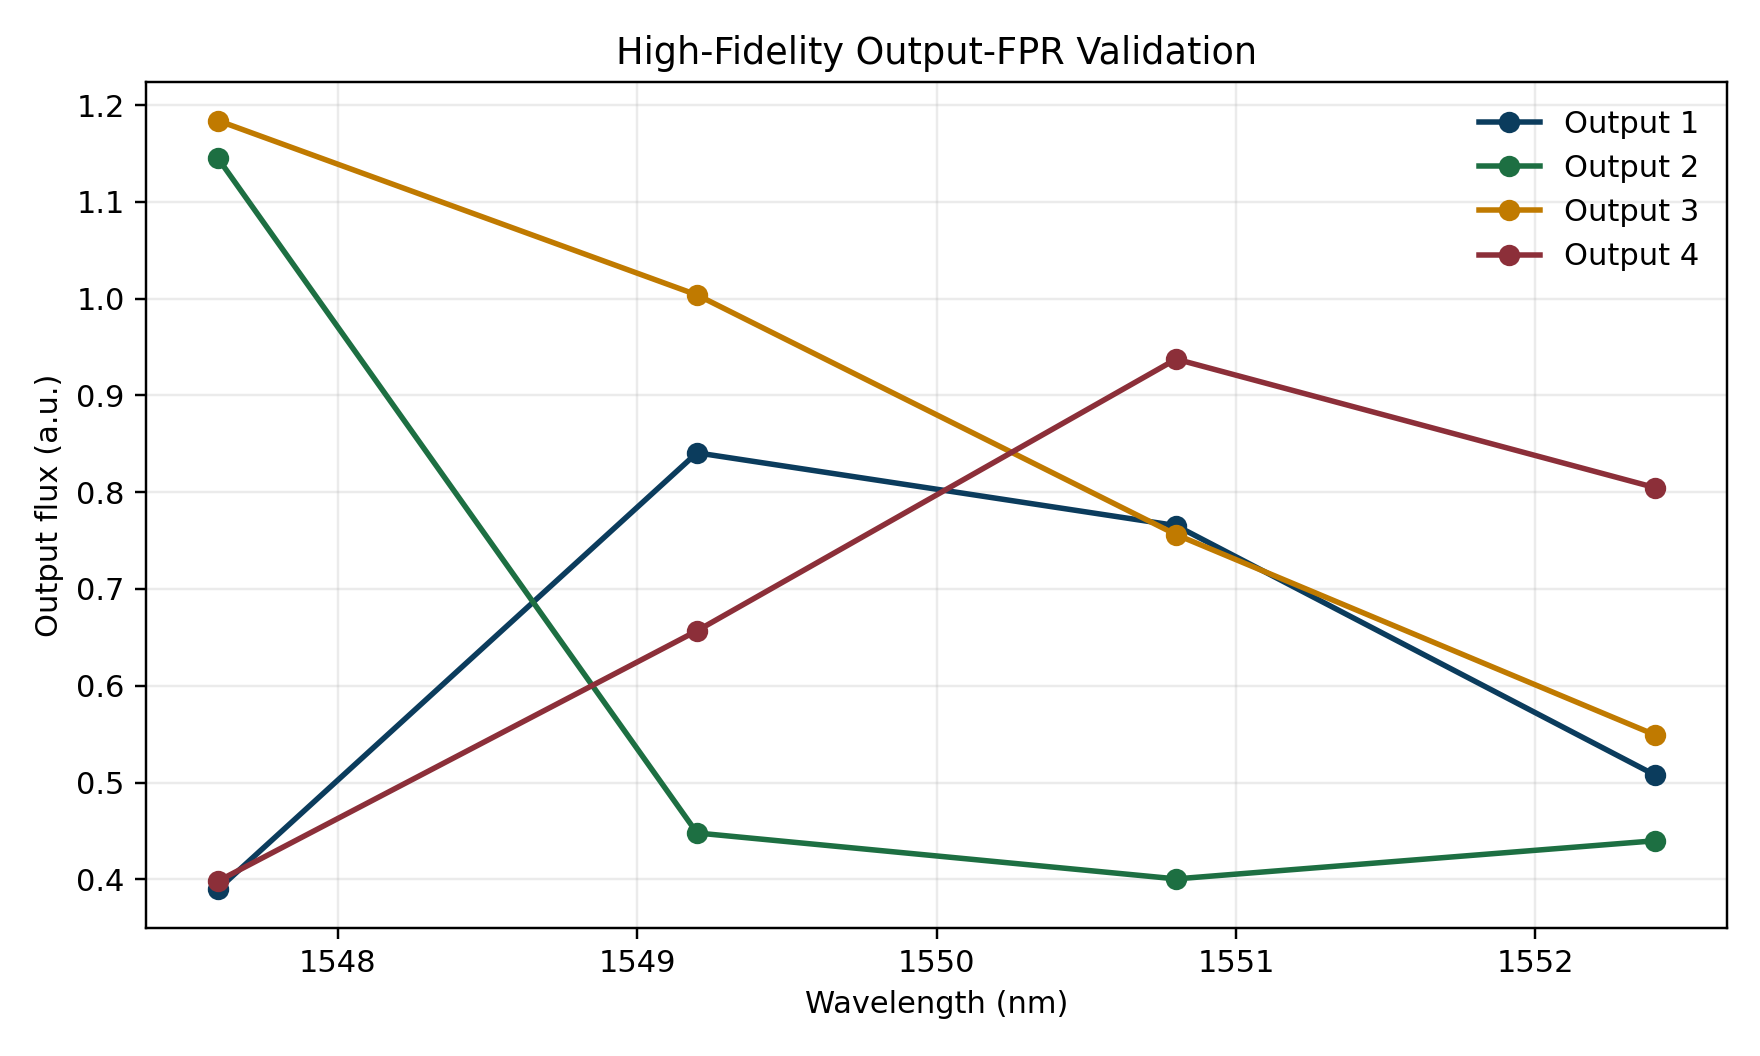
\includegraphics[width=\linewidth]{results/figures/awg_high_fidelity_transmission.png}
        {\footnotesize 各输出端口功率分布（Baseline，4个波长）}
      \end{center}
  \end{columns}
\end{frame}

% ── 第13页：全部优化轮次 ─────────────────────────────────────────────────────
\begin{frame}{优化过程：四轮改进}
  \begin{columns}[T]
    \column{0.48\textwidth}
      \small\textbf{第1--3轮：几何参数调整（N=16）}\\[3pt]
      \begin{center}
        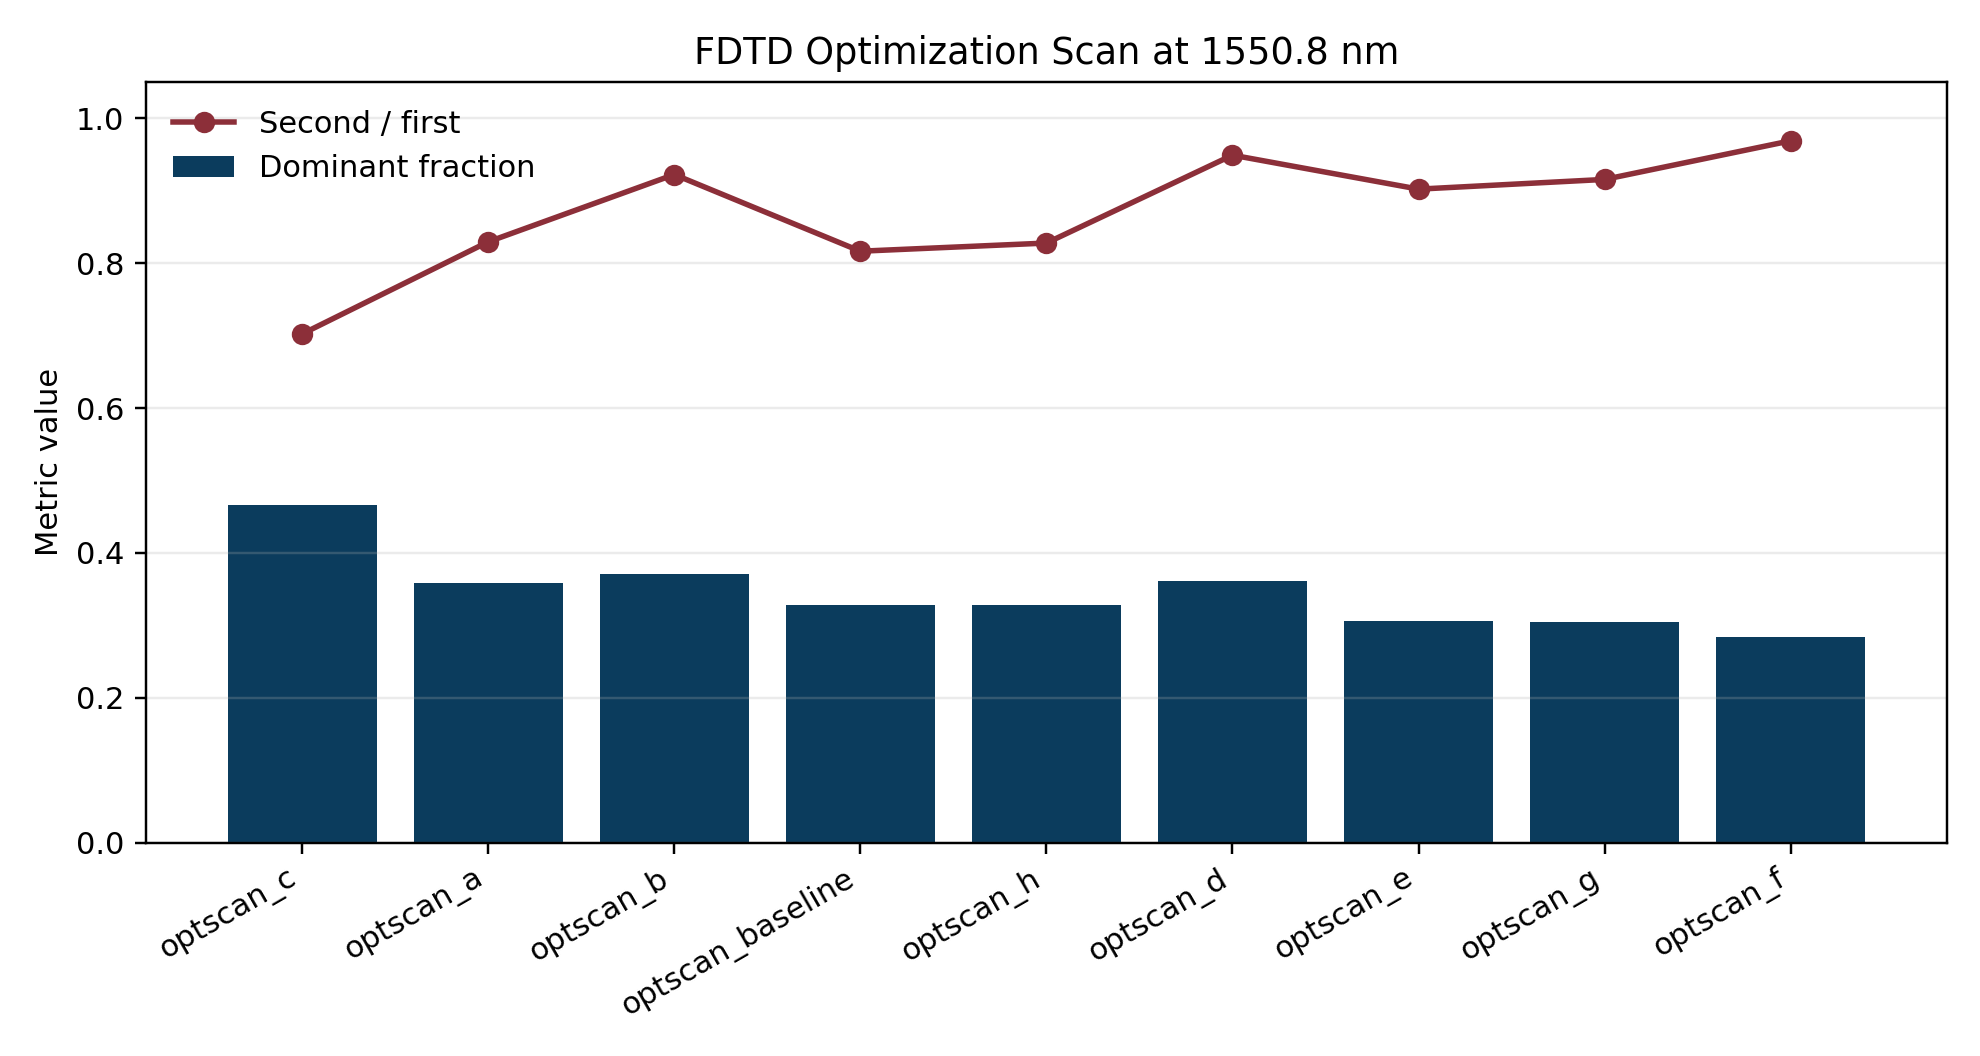
\includegraphics[width=0.95\linewidth]{results/figures/awg_hf_optimization_scan.png}
        {\footnotesize 9组配置在 1550.8\,nm 处扫描——optscan\_c 最优}
      \end{center}
      \small\textbf{N=16 最优：}阵距 $1.2\,\mu$m，输出距 $1.6\,\mu$m，偏移 $0.6\,\mu$m\\
      1550.8\,nm：合格(0.328)$\to$\textbf{良(0.466)}\\[2pt]
      \textit{瓶颈：3dB 带宽 1.2\,nm $\approx$ 间距 1.6\,nm，重叠严重}

    \column{0.49\textwidth}
      \small\textbf{第4轮：N=24 臂——关键突破}
      \begin{center}
        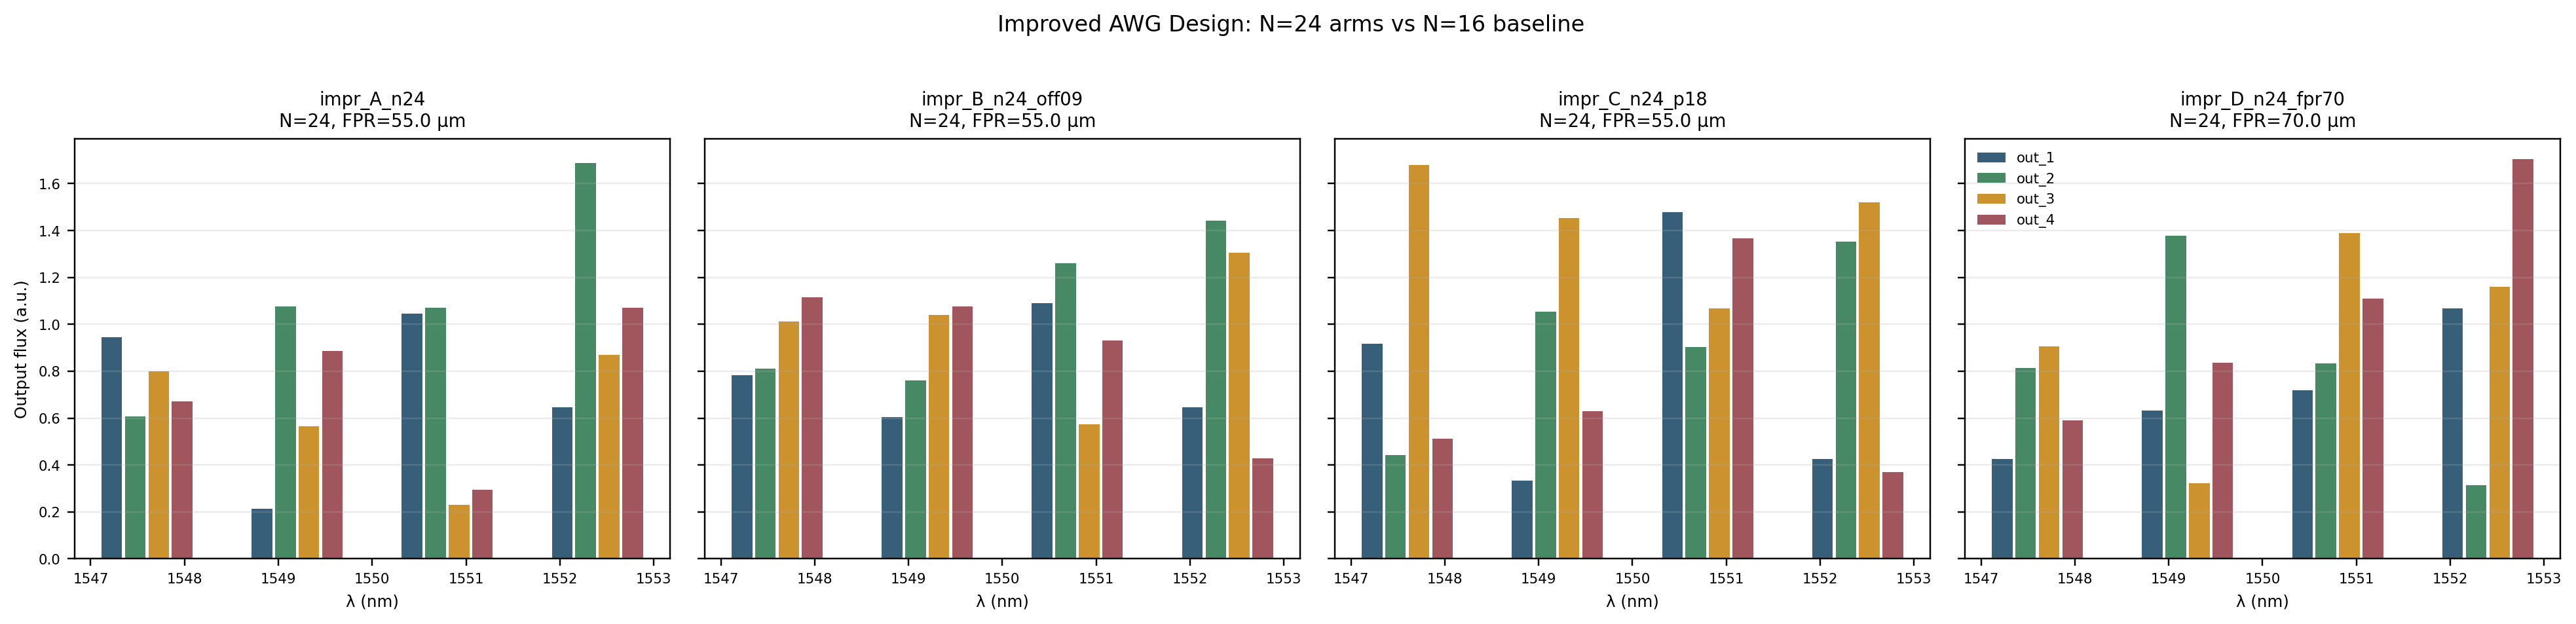
\includegraphics[width=0.95\linewidth]{results/figures/awg_improved_design_channels.png}
        {\footnotesize 4组 N=24 配置；impr\_C 总体最优}
      \end{center}
      \small impr\_C（输出距1.8，偏移0.9）：均值 0.403，\textbf{2个通道达到"良"}\\[2pt]
      3dB 带宽：$19.2/24 = 0.8$\,nm，现在远小于间距 $\checkmark$
  \end{columns}
\end{frame}

% ── 第14页：完整结果汇总 ─────────────────────────────────────────────────────
\begin{frame}{完整优化结果汇总}
  \begin{center}
  \small
  \renewcommand{\arraystretch}{1.35}
  \begin{tabular}{llccccc}
    \toprule
    \textbf{阶段} & \textbf{配置} &
    \textbf{均值占比} & \textbf{"良"通道数} & \textbf{最差次/主比} &
    \textbf{vs Baseline} \\
    \midrule
    Baseline   & N=16, 1.5/2.0/0.0 & 0.352 & 0 & 0.967 & — \\
    第1轮粗筛  & 本地375组扫描     & —     & — & —     & （筛选）\\
    第2轮局部  & N=16, 1.2/1.6/0.6 & 0.368 & 1 & 0.932 & $+$5\% \\
    第3轮全局  & N=16, 1.2/1.6/0.6 & 0.368 & 1 & 0.932 & $+$5\% \\
    \rowcolor{uw_gold!50}
    \textbf{第4轮 N=24} & \textbf{N=24, 1.2/1.8/0.9} & \textbf{0.403} &
    \textbf{2} & \textbf{0.924} & \textbf{$+$15\%} \\
    \bottomrule
  \end{tabular}
  \end{center}
  \vspace{4pt}
  \begin{columns}[T]
    \column{0.50\textwidth}
      \small\textbf{相比 Baseline 的累计改善：}
      \begin{itemize}\setlength\itemsep{2pt}
        \item 均值主输出占比：$0.352\to\mathbf{0.403}$ \;($+15\%$)
        \item 达到"良"的通道数：$0\to\mathbf{2}$
        \item 最差次/主比：$0.967\to\mathbf{0.924}$
      \end{itemize}
    \column{0.47\textwidth}
      \begin{block}{\small 核心教训}
        \small 几何调参（第2/3轮）收益有限。\\
        改变物理结构——增加臂数使 3dB 带宽变窄——\\
        是\textbf{单次改动效益最高的一步}。
      \end{block}
  \end{columns}
\end{frame}

% ── 第15页：结论与展望 ───────────────────────────────────────────────────────
\begin{frame}{结论与展望}
  \begin{columns}[T]
    \column{0.50\textwidth}
      \textbf{已完成的工作：}
      \begin{enumerate}\small\setlength\itemsep{3pt}
        \item 完整设计链：MODE $\to$ 参数 $\to$ FDTD $\to$ 优化
        \item 波长路由在真实麦克斯韦仿真中\textbf{得到证实}
        \item 3轮几何优化：中心波长达到\textbf{"良"}等级
        \item N=24 改进：2个通道达到"良"，均值 $+15\%$
        \item 延伸目标：8通道、温度 $+40$\,K、串扰改善——均有 FDTD 验证
      \end{enumerate}

    \column{0.47\textwidth}
      \textbf{当前局限：}
      \begin{itemize}\small\setlength\itemsep{3pt}
        \item 全4通道尚未整体达到"良"
        \item 矩形 FPR（非 Rowland 圆）导致 N=24 时中心通道偏弱
        \item 2D 模型忽略弯曲损耗和模式失配
      \end{itemize}
      \vspace{5pt}
      \textbf{后续方向（优先级）：}
      \begin{enumerate}\small\setlength\itemsep{2pt}
        \item N=24 细调偏移量（$\approx$0.3 FC）
        \item \textbf{Rowland 圆 FPR}——修复中心通道问题
        \item N=32 + FPR=90\,$\mu$m
        \item 完整 3D FDTD（获取准确插损/串扰数值）
      \end{enumerate}
  \end{columns}
  \vspace{6pt}
  \begin{center}\large\textbf{感谢聆听！欢迎提问。}\end{center}
\end{frame}

\end{document}
